\documentclass[11pt,a4paper]{article}

% Packages
\usepackage[margin=2.5cm]{geometry}
\usepackage{microtype}
\usepackage{graphicx}
\usepackage{tikz}
\usetikzlibrary{shapes,arrows.meta,positioning,calc,fit,backgrounds,shadows.blur,decorations.pathmorphing,decorations.pathreplacing}
\usepackage{colortbl}
\usepackage{enumitem}
\usepackage{booktabs}
\usepackage{longtable}
\usepackage{hyperref}
\usepackage{xcolor}
\usepackage{fancyhdr}
\usepackage{titlesec}
\usepackage[most]{tcolorbox}
\usepackage{multicol}
\usepackage{amsmath,amssymb}
\usepackage{multirow}
\usepackage{setspace}
\usepackage{fontawesome5}
\usepackage{listings}

% Spacing
\setlength{\parskip}{3pt plus 1pt minus 1pt}
\setlength{\parindent}{0pt}

% Colors
\definecolor{primary}{HTML}{1A5276}
\definecolor{secondary}{HTML}{2E86C1}
\definecolor{accent}{HTML}{E74C3C}
\definecolor{lightbg}{HTML}{EBF5FB}
\definecolor{defbg}{HTML}{FDF2E9}
\definecolor{greenhl}{HTML}{27AE60}
\definecolor{purplehl}{HTML}{8E44AD}
\definecolor{codebg}{HTML}{F4F6F7}

% Hyperref
\hypersetup{colorlinks=true, linkcolor=primary, urlcolor=secondary, citecolor=primary}

% Code listings style
\lstset{
  backgroundcolor=\color{codebg},
  basicstyle=\ttfamily\small,
  keywordstyle=\color{primary}\bfseries,
  stringstyle=\color{greenhl},
  commentstyle=\color{gray},
  breaklines=true,
  frame=l,
  framerule=2pt,
  rulecolor=\color{secondary!40},
  xleftmargin=8pt,
  framexleftmargin=6pt,
  aboveskip=6pt,
  belowskip=6pt
}

% Header/Footer
\pagestyle{fancy}
\fancyhf{}
\fancyhead[L]{\small\textcolor{primary}{\textbf{Machine Learning --- Fundamentals to Practice}}}
\fancyhead[R]{\small\textcolor{primary}{Lecture Handout}}
\fancyfoot[C]{\small\thepage}
\renewcommand{\headrulewidth}{0.5pt}
\renewcommand{\footrulewidth}{0.3pt}

% Section formatting
\titleformat{\section}{\Large\bfseries\color{primary}}{\thesection}{0.6em}{}[\vspace{2pt}\titlerule]
\titleformat{\subsection}{\large\bfseries\color{secondary}}{\thesubsection}{0.5em}{}
\titleformat{\subsubsection}{\normalsize\bfseries\color{primary}}{\thesubsubsection}{0.5em}{}
\titlespacing*{\section}{0pt}{14pt}{8pt}
\titlespacing*{\subsection}{0pt}{10pt}{5pt}

% Custom boxes
\newtcolorbox{definitionbox}[1][]{
  enhanced, breakable,
  colback=defbg, colframe=orange!60!black,
  colbacktitle=orange!70!black, coltitle=white,
  title={\faIcon{book}~#1}, fonttitle=\bfseries,
  boxrule=0pt, leftrule=4pt, arc=2pt,
  shadow={1mm}{-1mm}{0mm}{black!15},
  top=4pt, bottom=4pt, left=8pt, right=8pt
}
\newtcolorbox{conceptbox}[1][]{
  enhanced, breakable,
  colback=lightbg, colframe=secondary,
  colbacktitle=secondary, coltitle=white,
  title={\faIcon{lightbulb}~#1}, fonttitle=\bfseries,
  boxrule=0pt, leftrule=4pt, arc=2pt,
  shadow={1mm}{-1mm}{0mm}{black!15},
  top=4pt, bottom=4pt, left=8pt, right=8pt
}
\newtcolorbox{alertbox}[1][]{
  enhanced, breakable,
  colback=red!4, colframe=accent,
  colbacktitle=accent, coltitle=white,
  title={\faIcon{exclamation-triangle}~#1}, fonttitle=\bfseries,
  boxrule=0pt, leftrule=4pt, arc=2pt,
  shadow={1mm}{-1mm}{0mm}{black!12},
  top=3pt, bottom=3pt, left=8pt, right=8pt
}
\newtcolorbox{examplebox}[1][]{
  enhanced, breakable,
  colback=green!4, colframe=greenhl,
  colbacktitle=greenhl, coltitle=white,
  title={\faIcon{code}~#1}, fonttitle=\bfseries,
  boxrule=0pt, leftrule=4pt, arc=2pt,
  shadow={1mm}{-1mm}{0mm}{black!12},
  top=3pt, bottom=3pt, left=8pt, right=8pt
}

\begin{document}

% Title
\begin{center}
\vspace*{0.5cm}
{\Huge\bfseries\textcolor{primary}{Machine Learning}}\\[8pt]
{\Huge\bfseries\textcolor{primary}{Fundamentals to Practice}}\\[16pt]
{\color{secondary}\rule{0.6\textwidth}{1.5pt}}\\[14pt]
{\Large\textsc{Comprehensive Lecture Handout}}\\[8pt]
{\large\textcolor{gray!70!black}{Concepts $\bullet$ Algorithms $\bullet$ Evaluation $\bullet$ Applications}}
\vspace{0.3cm}
\end{center}
\tableofcontents
\newpage

%=============================================================
\section{Introduction to Machine Learning}
%=============================================================

\begin{definitionbox}[Machine Learning]
A subfield of Artificial Intelligence (AI) that gives computers the ability to \textbf{learn from data} and make predictions or decisions \textbf{without being explicitly programmed} for every scenario.\\[4pt]
\textit{``A computer program is said to learn from experience E with respect to some task T and some performance measure P, if its performance on T, as measured by P, improves with experience E.''} --- Tom Mitchell (1997)
\end{definitionbox}

\subsection{Where ML Fits: AI Landscape}

\begin{center}
\begin{tikzpicture}[scale=1]
  % Drop shadow
  \fill[black!8] (0.08,-0.08) circle (4.5cm);
  % Outermost circle - AI
  \fill[blue!6] (0,0) circle (4.5cm);
  \draw[thick, primary, line width=1.5pt] (0,0) circle (4.5cm);
  \node[font=\bfseries\large, primary] at (0,3.85) {\faIcon{robot}~Artificial Intelligence};
  \node[font=\scriptsize, primary!70, align=center] at (3.2,-3.2) {Rule-based systems,\\Expert systems,\\Search, Planning};

  % Middle circle - Machine Learning
  \fill[orange!8] (0,-0.4) circle (2.9cm);
  \draw[thick, orange!70!black, line width=1.2pt] (0,-0.4) circle (2.9cm);
  \node[font=\bfseries, orange!70!black] at (0,2.0) {\faIcon{brain}~Machine Learning};
  \node[font=\scriptsize, orange!50!black, align=center] at (-2.2,0.3) {Statistical\\learning,\\Pattern\\recognition};

  % Inner circle - Deep Learning
  \fill[green!8] (0,-0.7) circle (1.5cm);
  \draw[thick, greenhl!70!black, line width=1.2pt] (0,-0.7) circle (1.5cm);
  \node[font=\bfseries\small, greenhl!70!black, align=center] at (0,-0.7) {\faIcon{project-diagram}\\Deep\\Learning};
\end{tikzpicture}
\end{center}
\smallskip
\begin{itemize}[leftmargin=1.5em, itemsep=3pt]
  \item \textbf{\textcolor{primary}{AI}} is the broadest field---any technique enabling machines to mimic human intelligence.
  \item \textbf{\textcolor{orange!70!black}{Machine Learning}} is a subset of AI that learns patterns from data automatically.
  \item \textbf{\textcolor{greenhl!70!black}{Deep Learning}} is a subset of ML using neural networks with many layers.
\end{itemize}

\subsection{Why Machine Learning?}
\begin{itemize}[leftmargin=*]
  \item Problems too complex to program explicitly (e.g., image recognition, language translation).
  \item Automatically adapts to new data without manual reprogramming.
  \item Discovers hidden patterns in large datasets that humans cannot easily find.
  \item Powers modern applications: search engines, recommendations, self-driving cars, medical diagnosis.
\end{itemize}

%=============================================================
\section{Types of Machine Learning}
%=============================================================

\begin{center}
\begin{tikzpicture}[scale=0.92, transform shape,
  box/.style={rectangle, draw, thick, fill=#1, minimum width=3.2cm, minimum height=1.1cm, align=center, font=\small\bfseries, rounded corners=4pt,
    blur shadow={shadow blur steps=5, shadow xshift=0.5mm, shadow yshift=-0.5mm}},
  child/.style={rectangle, draw, thick, fill=#1, minimum width=2.6cm, minimum height=0.85cm, align=center, font=\scriptsize\bfseries, rounded corners=3pt,
    blur shadow={shadow blur steps=3, shadow xshift=0.3mm, shadow yshift=-0.3mm}},
  arr/.style={-{Stealth}, thick, primary!60}
]
  % Root
  \node[box=primary!15] (ml) at (0,0) {\faIcon{brain}\\Machine Learning};

  % Three branches
  \node[box=blue!12] (sup) at (-5.5,-2.5) {\faIcon{chalkboard-teacher}\\Supervised\\Learning};
  \node[box=orange!12] (unsup) at (0,-2.5) {\faIcon{search}\\Unsupervised\\Learning};
  \node[box=green!12] (rl) at (5.5,-2.5) {\faIcon{gamepad}\\Reinforcement\\Learning};

  \draw[arr] (ml) -- (sup);
  \draw[arr] (ml) -- (unsup);
  \draw[arr] (ml) -- (rl);

  % Supervised children
  \node[child=blue!8] (cls) at (-7.2,-4.7) {Classification};
  \node[child=blue!8] (reg) at (-3.8,-4.7) {Regression};
  \draw[arr] (sup) -- (cls);
  \draw[arr] (sup) -- (reg);

  % Unsupervised children
  \node[child=orange!8] (clust) at (-1.6,-4.7) {Clustering};
  \node[child=orange!8, minimum width=3.0cm] (dim) at (1.8,-4.7) {Dimensionality\\Reduction};
  \draw[arr] (unsup) -- (clust);
  \draw[arr] (unsup) -- (dim);

  % RL children
  \node[child=green!8] (pol) at (4.0,-4.7) {Policy-Based};
  \node[child=green!8] (val) at (7.0,-4.7) {Value-Based};
  \draw[arr] (rl) -- (pol);
  \draw[arr] (rl) -- (val);
\end{tikzpicture}
\end{center}

\subsection{Supervised Learning}
\begin{definitionbox}[Supervised Learning]
The algorithm learns from \textbf{labeled training data}---input-output pairs $(x_i, y_i)$---to learn a mapping function $f: X \rightarrow Y$ that can predict outputs for new, unseen inputs.
\end{definitionbox}

\begin{itemize}[leftmargin=*]
  \item \textbf{Classification:} Predicting a \emph{discrete} class label.\\
    \textit{Examples:} Spam detection (spam/not spam), disease diagnosis (positive/negative), image recognition (cat/dog).
  \item \textbf{Regression:} Predicting a \emph{continuous} numerical value.\\
    \textit{Examples:} House price prediction, stock price forecasting, temperature prediction.
\end{itemize}

\subsection{Unsupervised Learning}
\begin{definitionbox}[Unsupervised Learning]
The algorithm learns from \textbf{unlabeled data}---finding hidden patterns, structures, or groupings in the data without predefined outputs.
\end{definitionbox}

\begin{itemize}[leftmargin=*]
  \item \textbf{Clustering:} Grouping similar data points together.\\
    \textit{Examples:} Customer segmentation, document grouping, anomaly detection.
  \item \textbf{Dimensionality Reduction:} Reducing the number of features while preserving important information.\\
    \textit{Examples:} PCA, t-SNE, autoencoders---used for visualization and noise reduction.
  \item \textbf{Association Rule Learning:} Finding interesting relationships between variables.\\
    \textit{Examples:} Market basket analysis (``customers who bought X also bought Y'').
\end{itemize}

\subsection{Reinforcement Learning}
\begin{definitionbox}[Reinforcement Learning]
An agent learns to make decisions by performing \textbf{actions} in an \textbf{environment} to maximize cumulative \textbf{reward}. It learns through trial and error.
\end{definitionbox}

\begin{center}
\begin{tikzpicture}[
  box/.style={rectangle, draw, thick, fill=#1, minimum width=2.6cm, minimum height=1.2cm, align=center, font=\small\bfseries, rounded corners=4pt,
    blur shadow={shadow blur steps=5, shadow xshift=0.5mm, shadow yshift=-0.5mm}},
  arr/.style={-{Stealth[length=3mm]}, very thick, line width=1.5pt}
]
  \node[box=blue!15] (agent) at (0,0) {\faIcon{user-cog}\\Agent};
  \node[box=green!15] (env) at (7,0) {\faIcon{globe}\\Environment};

  \draw[arr, primary!70] (agent.north east) -- node[above, font=\small] {Action $a_t$} (env.north west);
  \draw[arr, greenhl!70] (env.south west) -- node[below, font=\small, align=center] {State $s_{t+1}$, Reward $r_{t+1}$} (agent.south east);
\end{tikzpicture}
\end{center}
\smallskip
\textit{Examples:} Game playing (AlphaGo, Atari), robotics, autonomous driving, recommendation systems.

\subsection{Semi-Supervised and Self-Supervised Learning}
\begin{itemize}[leftmargin=*]
  \item \textbf{Semi-Supervised:} Uses a small amount of labeled data combined with a large amount of unlabeled data.
  \item \textbf{Self-Supervised:} The model generates its own labels from the data (e.g., predicting the next word in a sentence). Foundation for large language models (GPT, BERT).
\end{itemize}

%=============================================================
\section{Key Terminology and Concepts}
%=============================================================

\rowcolors{2}{white}{defbg}
\begin{longtable}{@{}p{3.5cm}p{10cm}@{}}
\toprule
\rowcolor{primary!15}
\textbf{Term} & \textbf{Definition} \\
\midrule
\endhead
Feature (Variable) & An individual measurable property of the data (input column), e.g., age, income, pixel value. \\
\addlinespace
Label (Target) & The output variable the model is trying to predict, e.g., spam/not spam, price. \\
\addlinespace
Training Set & The portion of data used to train (fit) the model. \\
\addlinespace
Validation Set & Data used to tune hyperparameters and prevent overfitting during training. \\
\addlinespace
Test Set & Held-out data used to evaluate the final model's performance on unseen data. \\
\addlinespace
Model & The mathematical function learned from data that maps inputs to outputs. \\
\addlinespace
Hyperparameter & A parameter set \emph{before} training (e.g., learning rate, number of trees, $k$ in KNN). \\
\addlinespace
Parameter & A value learned \emph{during} training (e.g., weights in linear regression, neural network weights). \\
\addlinespace
Epoch & One complete pass through the entire training dataset. \\
\addlinespace
Batch Size & Number of training samples used in one iteration of model update. \\
\addlinespace
Loss Function & A function that measures how far the model's predictions are from actual values. \\
\addlinespace
Gradient Descent & An optimization algorithm that iteratively adjusts parameters to minimize the loss function. \\
\bottomrule
\end{longtable}

%=============================================================
\section{The Machine Learning Pipeline}
%=============================================================

\begin{center}
\begin{tikzpicture}[
  step/.style={rectangle, draw, thick, fill=#1, minimum width=2.1cm, minimum height=1.3cm, align=center, font=\footnotesize\bfseries, rounded corners=4pt,
    blur shadow={shadow blur steps=5, shadow xshift=0.5mm, shadow yshift=-0.5mm}},
  arr/.style={-{Stealth[length=2.5mm]}, very thick, primary!60, line width=1.2pt}
]
  \node[step=blue!12]   (s1) at (0,0)    {\faIcon{database}\\Data\\Collection};
  \node[step=cyan!12]   (s2) at (2.7,0)  {\faIcon{broom}\\Data\\Cleaning};
  \node[step=orange!12] (s3) at (5.4,0)  {\faIcon{cogs}\\Feature\\Engineering};
  \node[step=yellow!15] (s4) at (8.1,0)  {\faIcon{cut}\\Train/Test\\Split};
  \node[step=green!12]  (s5) at (10.8,0) {\faIcon{brain}\\Model\\Training};
  \node[step=red!10]    (s6) at (8.1,-2.5) {\faIcon{chart-bar}\\Model\\Evaluation};
  \node[step=purple!12] (s7) at (5.4,-2.5) {\faIcon{sliders-h}\\Hyper-\\parameter\\Tuning};
  \node[step=primary!12](s8) at (2.7,-2.5) {\faIcon{rocket}\\Deploy-\\ment};

  \draw[arr] (s1) -- (s2);
  \draw[arr] (s2) -- (s3);
  \draw[arr] (s3) -- (s4);
  \draw[arr] (s4) -- (s5);
  \draw[arr] (s5) -- (s6);
  \draw[arr] (s6) -- (s7);
  \draw[arr] (s7) -- (s8);
  % Feedback loop
  \draw[arr, dashed, secondary] (s7.north) to[bend left=30] node[above, font=\tiny\itshape, secondary] {retrain} (s5.south);
\end{tikzpicture}
\end{center}

\subsection{Step 1: Data Collection}
Gather data from databases, APIs, web scraping, sensors, surveys, or public datasets. Quality and quantity of data directly impact model performance.

\subsection{Step 2: Data Cleaning and Preprocessing}
\begin{itemize}[leftmargin=*]
  \item \textbf{Handle missing values:} Imputation (mean, median, mode), removal, or advanced methods (KNN imputation).
  \item \textbf{Remove duplicates} and correct inconsistent entries.
  \item \textbf{Handle outliers:} IQR method, Z-score, domain knowledge.
  \item \textbf{Data type conversions:} Ensure proper types (numeric, categorical, datetime).
\end{itemize}

\subsection{Step 3: Feature Engineering}
\begin{definitionbox}[Feature Engineering]
The process of transforming raw data into meaningful features that better represent the underlying problem, improving model accuracy.
\end{definitionbox}
\begin{itemize}[leftmargin=*]
  \item \textbf{Encoding categorical variables:} One-hot encoding, label encoding, target encoding.
  \item \textbf{Feature scaling:} Standardization ($z = \frac{x - \mu}{\sigma}$) or Min-Max normalization ($x' = \frac{x - x_{\min}}{x_{\max} - x_{\min}}$).
  \item \textbf{Feature creation:} Polynomial features, interaction terms, domain-specific features.
  \item \textbf{Feature selection:} Removing irrelevant or redundant features (correlation analysis, mutual information, recursive feature elimination).
\end{itemize}

\subsection{Step 4: Train/Test Split}
\begin{conceptbox}[Data Splitting]
Typically split data into \textbf{training set} (70--80\%) and \textbf{test set} (20--30\%). For hyperparameter tuning, further split training data into training and \textbf{validation set}, or use \textbf{cross-validation}.
\end{conceptbox}

\subsection{Step 5--7: Training, Evaluation, Tuning}
These are detailed in the following sections.

%=============================================================
\section{Supervised Learning Algorithms}
%=============================================================

\subsection{Linear Regression}

\begin{definitionbox}[Linear Regression]
Models the relationship between a dependent variable $y$ and one or more independent variables $x$ by fitting a linear equation:
$$\hat{y} = w_0 + w_1 x_1 + w_2 x_2 + \cdots + w_n x_n = \mathbf{w}^T \mathbf{x} + b$$
Minimizes the \textbf{Mean Squared Error (MSE)}: $\text{MSE} = \frac{1}{n}\sum_{i=1}^{n}(y_i - \hat{y}_i)^2$
\end{definitionbox}

\begin{center}
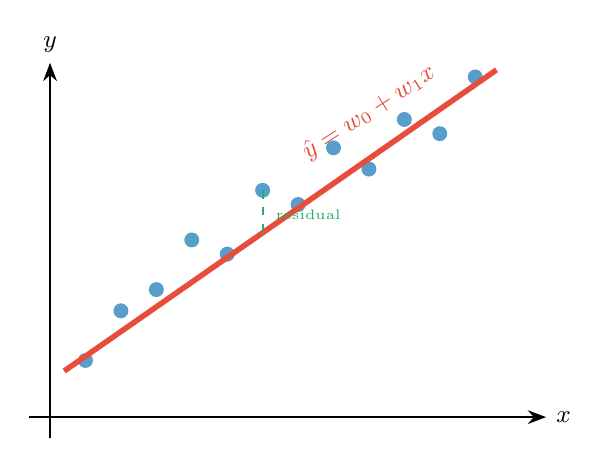
\begin{tikzpicture}[scale=0.9]
  \draw[-{Stealth}, thick] (-0.3,0) -- (7,0) node[right, font=\small] {$x$};
  \draw[-{Stealth}, thick] (0,-0.3) -- (0,5) node[above, font=\small] {$y$};
  % Data points
  \foreach \x/\y in {0.5/0.8, 1.0/1.5, 1.5/1.8, 2.0/2.5, 2.5/2.3, 3.0/3.2, 3.5/3.0, 4.0/3.8, 4.5/3.5, 5.0/4.2, 5.5/4.0, 6.0/4.8} {
    \fill[secondary!80] (\x, \y) circle (3pt);
  }
  % Regression line
  \draw[very thick, accent, line width=2pt] (0.2, 0.65) -- (6.3, 4.9);
  \node[font=\small\bfseries, accent, rotate=33] at (4.5, 4.3) {$\hat{y} = w_0 + w_1 x$};
  % Residual example
  \draw[dashed, greenhl, thick] (3.0, 3.2) -- (3.0, 2.55);
  \node[font=\tiny, greenhl, right] at (3.05, 2.85) {residual};
\end{tikzpicture}
\end{center}

\begin{itemize}[leftmargin=*]
  \item \textbf{Assumptions:} Linearity, independence, homoscedasticity, normality of residuals.
  \item \textbf{Regularization:} Ridge (L2: $+\lambda\sum w_i^2$), Lasso (L1: $+\lambda\sum |w_i|$), Elastic Net (L1 + L2).
\end{itemize}

\subsection{Logistic Regression}

\begin{definitionbox}[Logistic Regression]
A classification algorithm that models the probability of a binary outcome using the \textbf{sigmoid function}:
$$P(y=1 \mid x) = \sigma(\mathbf{w}^T\mathbf{x} + b) = \frac{1}{1 + e^{-(\mathbf{w}^T\mathbf{x} + b)}}$$
Output is a probability between 0 and 1; a threshold (typically 0.5) determines the class.
\end{definitionbox}

\begin{center}
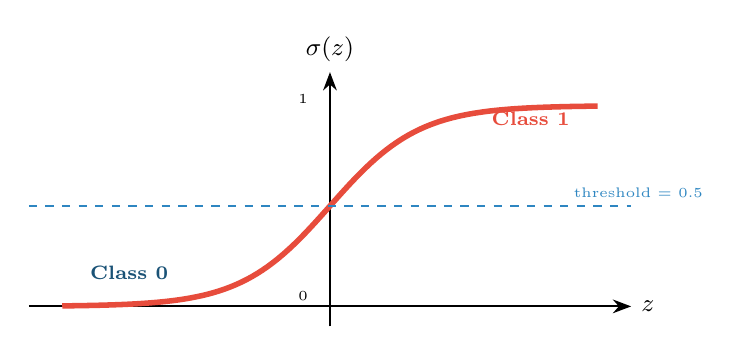
\begin{tikzpicture}[scale=0.85]
  \draw[-{Stealth}, thick] (-4.5,0) -- (4.5,0) node[right, font=\small] {$z$};
  \draw[-{Stealth}, thick] (0,-0.3) -- (0,3.5) node[above, font=\small] {$\sigma(z)$};
  % Sigmoid curve
  \draw[very thick, accent, line width=2pt, domain=-4:4, samples=100] plot (\x, {3/(1+exp(-1.5*\x))});
  % Threshold line
  \draw[dashed, secondary, thick] (-4.5, 1.5) -- (4.5, 1.5);
  \node[font=\tiny, secondary, right] at (3.5, 1.7) {threshold = 0.5};
  % Labels
  \node[font=\tiny] at (-0.4, 3.1) {1};
  \node[font=\tiny] at (-0.4, 0.15) {0};
  \node[font=\scriptsize\bfseries, primary] at (-3, 0.5) {Class 0};
  \node[font=\scriptsize\bfseries, accent] at (3, 2.8) {Class 1};
\end{tikzpicture}
\end{center}

\subsection{Decision Trees}

\begin{definitionbox}[Decision Tree]
A tree-structured model that makes decisions by recursively splitting data based on feature values. Each internal node represents a test on a feature, each branch represents an outcome, and each leaf node represents a class label or value.
\end{definitionbox}

\begin{center}
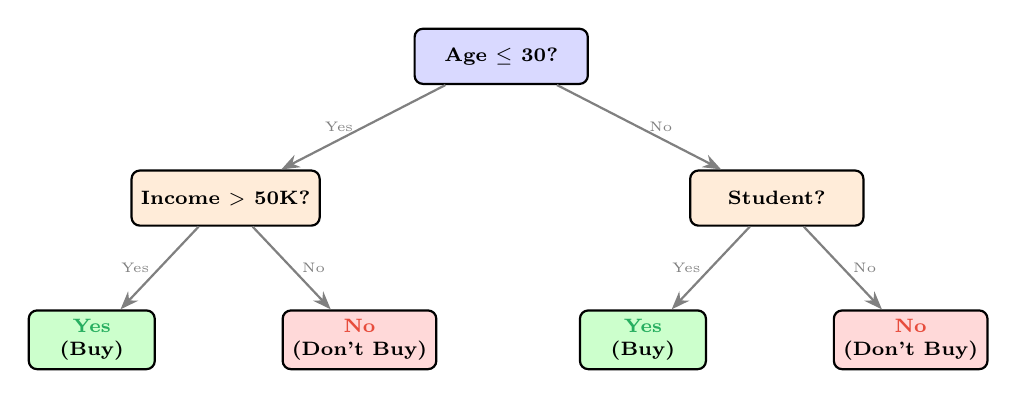
\begin{tikzpicture}[
  treenode/.style={rectangle, draw, thick, fill=#1, minimum width=2.2cm, minimum height=0.7cm, align=center, font=\scriptsize\bfseries, rounded corners=3pt},
  leaf/.style={rectangle, draw, thick, fill=#1, minimum width=1.6cm, minimum height=0.6cm, align=center, font=\scriptsize\bfseries, rounded corners=3pt},
  arr/.style={-{Stealth}, thick, black!50},
  level distance=1.6cm, sibling distance=3.5cm
]
  \node[treenode=blue!15] (root) {Age $\leq$ 30?};

  \node[treenode=orange!15] (l1) at (-3.5, -1.8) {Income $>$ 50K?};
  \node[treenode=orange!15] (r1) at (3.5, -1.8) {Student?};

  \node[leaf=green!20] (ll) at (-5.2, -3.6) {\textcolor{greenhl}{Yes}\\(Buy)};
  \node[leaf=red!15] (lr) at (-1.8, -3.6) {\textcolor{accent}{No}\\(Don't Buy)};
  \node[leaf=green!20] (rl) at (1.8, -3.6) {\textcolor{greenhl}{Yes}\\(Buy)};
  \node[leaf=red!15] (rr) at (5.2, -3.6) {\textcolor{accent}{No}\\(Don't Buy)};

  \draw[arr] (root) -- node[left, font=\tiny] {Yes} (l1);
  \draw[arr] (root) -- node[right, font=\tiny] {No} (r1);
  \draw[arr] (l1) -- node[left, font=\tiny] {Yes} (ll);
  \draw[arr] (l1) -- node[right, font=\tiny] {No} (lr);
  \draw[arr] (r1) -- node[left, font=\tiny] {Yes} (rl);
  \draw[arr] (r1) -- node[right, font=\tiny] {No} (rr);
\end{tikzpicture}
\end{center}

\begin{itemize}[leftmargin=*]
  \item \textbf{Splitting criteria:} Gini Impurity, Information Gain (Entropy), Variance Reduction.
  \item \textbf{Gini Impurity:} $G = 1 - \sum_{k=1}^{K} p_k^2$ \quad (lower is purer)
  \item \textbf{Entropy:} $H = -\sum_{k=1}^{K} p_k \log_2 p_k$
  \item \textbf{Pros:} Easy to interpret, handles both numerical and categorical data, no feature scaling needed.
  \item \textbf{Cons:} Prone to overfitting, unstable (small data changes $\rightarrow$ different trees).
\end{itemize}

\subsection{K-Nearest Neighbors (KNN)}

\begin{definitionbox}[KNN]
A \textbf{non-parametric, instance-based} algorithm that classifies a new data point based on the majority class of its $k$ nearest neighbors in the feature space.
\end{definitionbox}

\begin{itemize}[leftmargin=*]
  \item \textbf{Distance metrics:} Euclidean ($\sqrt{\sum(x_i - y_i)^2}$), Manhattan ($\sum|x_i - y_i|$), Minkowski.
  \item \textbf{Choosing $k$:} Small $k$ = high variance (overfitting); large $k$ = high bias (underfitting). Use cross-validation.
  \item \textbf{Pros:} Simple, no training phase, works with multi-class.
  \item \textbf{Cons:} Slow on large datasets, sensitive to feature scaling, curse of dimensionality.
\end{itemize}

\subsection{Support Vector Machines (SVM)}

\begin{definitionbox}[SVM]
Finds the optimal \textbf{hyperplane} that maximizes the \textbf{margin} (distance) between two classes. Support vectors are the data points closest to the hyperplane.
\end{definitionbox}

\begin{center}
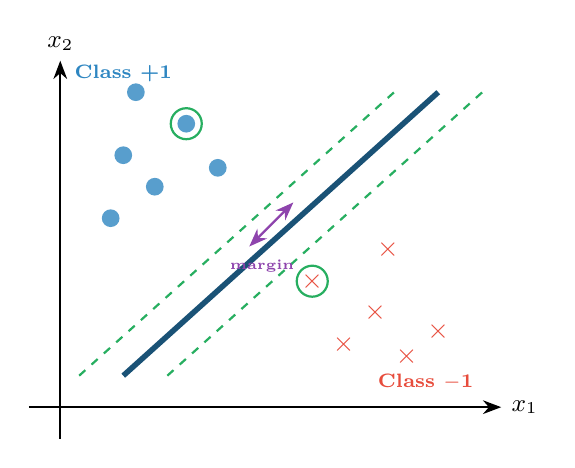
\begin{tikzpicture}[scale=0.8]
  \draw[-{Stealth}, thick] (-0.5,0) -- (7,0) node[right, font=\small] {$x_1$};
  \draw[-{Stealth}, thick] (0,-0.5) -- (0,5.5) node[above, font=\small] {$x_2$};

  % Class 1 points
  \foreach \x/\y in {1.0/4.0, 1.5/3.5, 0.8/3.0, 2.0/4.5, 1.2/5.0, 2.5/3.8} {
    \fill[secondary!80] (\x, \y) circle (4pt);
  }
  % Class 2 points
  \foreach \x/\y in {4.5/1.0, 5.0/1.5, 5.5/0.8, 4.0/2.0, 5.2/2.5, 6.0/1.2} {
    \node[accent, font=\bfseries] at (\x, \y) {$\times$};
  }

  % Decision boundary
  \draw[very thick, primary, line width=2pt] (1.0, 0.5) -- (6.0, 5.0);
  % Margin lines
  \draw[dashed, greenhl, thick] (0.3, 0.5) -- (5.3, 5.0);
  \draw[dashed, greenhl, thick] (1.7, 0.5) -- (6.7, 5.0);

  % Support vectors (circled)
  \draw[thick, greenhl] (2.0, 4.5) circle (7pt);
  \draw[thick, greenhl] (4.0, 2.0) circle (7pt);

  % Labels
  \node[font=\scriptsize\bfseries, secondary] at (1.0, 5.3) {Class +1};
  \node[font=\scriptsize\bfseries, accent] at (5.8, 0.4) {Class $-$1};
  \draw[{Stealth}-{Stealth}, thick, purplehl] (3.0, 2.55) -- (3.7, 3.25);
  \node[font=\tiny\bfseries, purplehl, below] at (3.2, 2.5) {margin};
\end{tikzpicture}
\end{center}

\begin{itemize}[leftmargin=*]
  \item \textbf{Kernel Trick:} Maps data to higher dimensions for non-linear separation. Common kernels: Linear, Polynomial, RBF (Gaussian).
  \item \textbf{Pros:} Effective in high dimensions, robust to overfitting (with proper regularization).
  \item \textbf{Cons:} Slow on very large datasets, requires feature scaling, not easily interpretable.
\end{itemize}

\subsection{Na\"ive Bayes}

\begin{definitionbox}[Na\"ive Bayes]
A probabilistic classifier based on \textbf{Bayes' Theorem} with a ``na\"ive'' assumption that all features are \textbf{conditionally independent} given the class:
$$P(C \mid X) = \frac{P(X \mid C) \cdot P(C)}{P(X)} \propto P(C) \prod_{i=1}^{n} P(x_i \mid C)$$
\end{definitionbox}

\begin{itemize}[leftmargin=*]
  \item \textbf{Variants:} Gaussian (continuous data), Multinomial (word counts), Bernoulli (binary features).
  \item \textbf{Pros:} Very fast, works well with high-dimensional data, excellent for text classification.
  \item \textbf{Cons:} Independence assumption rarely holds, poor probability estimates.
\end{itemize}

%=============================================================
\section{Ensemble Methods}
%=============================================================

\begin{conceptbox}[Ensemble Learning]
Combining multiple models to produce a stronger model than any individual one. The key idea: diverse models make different errors, and combining them reduces overall error.
\end{conceptbox}

\begin{center}
\begin{tikzpicture}[
  box/.style={rectangle, draw, thick, fill=#1, minimum width=2.4cm, minimum height=0.9cm, align=center, font=\scriptsize\bfseries, rounded corners=3pt,
    blur shadow={shadow blur steps=4, shadow xshift=0.4mm, shadow yshift=-0.4mm}},
  arr/.style={-{Stealth}, thick, primary!60}
]
  \node[box=primary!12] (data) at (0,0) {\faIcon{database}~Training Data};

  \node[box=blue!12] (m1) at (-3.5,-1.8) {Model 1};
  \node[box=blue!12] (m2) at (0,-1.8) {Model 2};
  \node[box=blue!12] (m3) at (3.5,-1.8) {Model $n$};
  \node[font=\large\bfseries, primary!40] at (1.75, -1.8) {$\cdots$};

  \node[box=green!15] (comb) at (0,-3.6) {\faIcon{layer-group}~Combine Predictions};
  \node[box=accent!12] (final) at (0,-5.2) {\faIcon{bullseye}~Final Prediction};

  \draw[arr] (data) -- (m1);
  \draw[arr] (data) -- (m2);
  \draw[arr] (data) -- (m3);
  \draw[arr] (m1) -- (comb);
  \draw[arr] (m2) -- (comb);
  \draw[arr] (m3) -- (comb);
  \draw[arr] (comb) -- (final);
\end{tikzpicture}
\end{center}

\subsection{Bagging (Bootstrap Aggregating)}
\begin{itemize}[leftmargin=*]
  \item Train multiple models on different \textbf{bootstrap samples} (random subsets with replacement).
  \item Combine via \textbf{majority voting} (classification) or \textbf{averaging} (regression).
  \item \textbf{Reduces variance}, helps prevent overfitting.
  \item \textbf{Key example: Random Forest.}
\end{itemize}

\begin{definitionbox}[Random Forest]
An ensemble of decision trees trained on bootstrap samples with \textbf{random feature subsets} at each split. Highly accurate, handles high-dimensional data, provides feature importance scores.
\end{definitionbox}

\subsection{Boosting}
\begin{itemize}[leftmargin=*]
  \item Train models \textbf{sequentially}---each new model focuses on the errors of the previous one.
  \item \textbf{Reduces bias and variance}.
  \item \textbf{Key algorithms:} AdaBoost, Gradient Boosting, XGBoost, LightGBM, CatBoost.
\end{itemize}

\begin{definitionbox}[Gradient Boosting]
Builds trees sequentially where each tree fits the \textbf{residual errors} (negative gradient of the loss function) of the previous ensemble. XGBoost, LightGBM, and CatBoost are highly optimized implementations widely used in competitions and industry.
\end{definitionbox}

\subsection{Bagging vs.\ Boosting}

\begin{center}
\begin{tabular}{@{}p{6.5cm}p{6.5cm}@{}}
\toprule
\textbf{Bagging (e.g., Random Forest)} & \textbf{Boosting (e.g., XGBoost)} \\
\midrule
Models trained in parallel & Models trained sequentially \\
Each model trained on bootstrap sample & Each model corrects predecessors' errors \\
Reduces variance & Reduces bias (and variance) \\
Less prone to overfitting & Can overfit if not regularized \\
Equal weight for all models & Models weighted by performance \\
\bottomrule
\end{tabular}
\end{center}

%=============================================================
\section{Unsupervised Learning Algorithms}
%=============================================================

\subsection{K-Means Clustering}

\begin{definitionbox}[K-Means]
Partitions $n$ data points into $k$ clusters by iteratively assigning points to the nearest \textbf{centroid} and updating centroids as the mean of assigned points. Minimizes \textbf{within-cluster sum of squares (WCSS)}.
\end{definitionbox}

\begin{center}
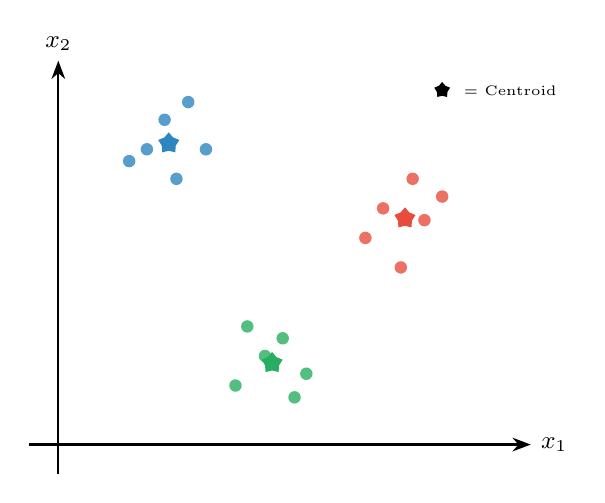
\begin{tikzpicture}[scale=0.75]
  \draw[-{Stealth}, thick] (-0.5,0) -- (8,0) node[right, font=\small] {$x_1$};
  \draw[-{Stealth}, thick] (0,-0.5) -- (0,6.5) node[above, font=\small] {$x_2$};

  % Cluster 1 (blue)
  \foreach \x/\y in {1.5/5.0, 2.0/4.5, 1.8/5.5, 2.5/5.0, 1.2/4.8, 2.2/5.8} {
    \fill[secondary!80] (\x, \y) circle (3pt);
  }
  \node[star, star points=5, fill=secondary, minimum size=8pt, inner sep=0pt] at (1.87, 5.1) {};

  % Cluster 2 (red)
  \foreach \x/\y in {5.5/4.0, 6.0/4.5, 5.2/3.5, 6.5/4.2, 5.8/3.0, 6.2/3.8} {
    \fill[accent!80] (\x, \y) circle (3pt);
  }
  \node[star, star points=5, fill=accent, minimum size=8pt, inner sep=0pt] at (5.87, 3.83) {};

  % Cluster 3 (green)
  \foreach \x/\y in {3.0/1.0, 3.5/1.5, 4.0/0.8, 3.2/2.0, 4.2/1.2, 3.8/1.8} {
    \fill[greenhl!80] (\x, \y) circle (3pt);
  }
  \node[star, star points=5, fill=greenhl, minimum size=8pt, inner sep=0pt] at (3.62, 1.38) {};

  % Legend
  \node[star, star points=5, fill=black, minimum size=6pt, inner sep=0pt] at (6.5, 6.0) {};
  \node[font=\tiny, right] at (6.7, 6.0) {= Centroid};
\end{tikzpicture}
\end{center}

\textbf{Algorithm steps:}
\begin{enumerate}[leftmargin=*]
  \item Choose $k$ (number of clusters).
  \item Randomly initialize $k$ centroids.
  \item Assign each point to the nearest centroid.
  \item Recompute centroids as mean of assigned points.
  \item Repeat steps 3--4 until convergence.
\end{enumerate}

\begin{itemize}[leftmargin=*]
  \item \textbf{Choosing $k$:} Elbow method (plot WCSS vs.\ $k$), Silhouette score.
  \item \textbf{Pros:} Simple, fast, scalable. \quad \textbf{Cons:} Assumes spherical clusters, sensitive to initialization and outliers.
\end{itemize}

\subsection{Hierarchical Clustering}
\begin{itemize}[leftmargin=*]
  \item \textbf{Agglomerative (bottom-up):} Start with each point as its own cluster; merge closest pairs iteratively.
  \item \textbf{Divisive (top-down):} Start with one cluster; recursively split.
  \item Visualized using a \textbf{dendrogram}; cut at desired level to get $k$ clusters.
  \item \textbf{Linkage methods:} Single, complete, average, Ward's.
\end{itemize}

\subsection{Principal Component Analysis (PCA)}

\begin{definitionbox}[PCA]
A dimensionality reduction technique that transforms data into a new coordinate system of \textbf{principal components}---orthogonal directions that capture the maximum variance.
$$\text{PC}_1 = w_1 x_1 + w_2 x_2 + \cdots + w_n x_n$$
The first principal component explains the most variance, the second the next most, etc.
\end{definitionbox}

\begin{itemize}[leftmargin=*]
  \item \textbf{Uses:} Visualization (reduce to 2D/3D), noise reduction, speeding up other algorithms, handling multicollinearity.
  \item \textbf{Steps:} Standardize data $\rightarrow$ Compute covariance matrix $\rightarrow$ Compute eigenvectors/eigenvalues $\rightarrow$ Select top $k$ components.
\end{itemize}

%=============================================================
\section{Neural Networks and Deep Learning}
%=============================================================

\begin{definitionbox}[Artificial Neural Network (ANN)]
A computational model inspired by the human brain, consisting of layers of interconnected \textbf{neurons} (nodes). Each connection has a \textbf{weight}, and each neuron applies an \textbf{activation function} to its weighted input sum.
\end{definitionbox}

\begin{center}
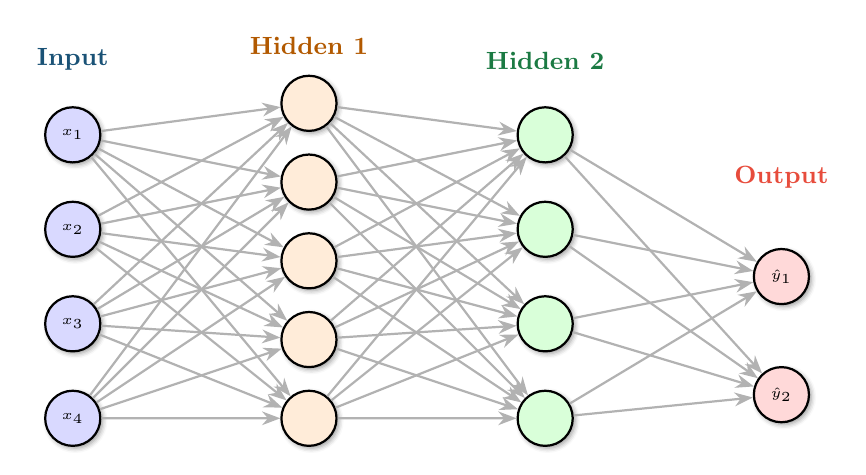
\begin{tikzpicture}[
  neuron/.style={circle, draw, thick, fill=#1, minimum size=0.7cm, font=\tiny\bfseries,
    blur shadow={shadow blur steps=4, shadow xshift=0.3mm, shadow yshift=-0.3mm}},
  arr/.style={-{Stealth}, thick, black!30}
]
  % Input layer
  \foreach \i in {1,2,3,4} {
    \node[neuron=blue!15] (i\i) at (0, -\i*1.2+3) {$x_{\i}$};
  }
  % Hidden layer 1
  \foreach \j in {1,2,3,4,5} {
    \node[neuron=orange!15] (h1\j) at (3, -\j*1.0+3.2) {};
  }
  % Hidden layer 2
  \foreach \j in {1,2,3,4} {
    \node[neuron=green!15] (h2\j) at (6, -\j*1.2+3) {};
  }
  % Output layer
  \foreach \k in {1,2} {
    \node[neuron=red!15] (o\k) at (9, -\k*1.5+1.5) {$\hat{y}_{\k}$};
  }

  % Connections
  \foreach \i in {1,2,3,4} {
    \foreach \j in {1,2,3,4,5} {
      \draw[arr] (i\i) -- (h1\j);
    }
  }
  \foreach \i in {1,2,3,4,5} {
    \foreach \j in {1,2,3,4} {
      \draw[arr] (h1\i) -- (h2\j);
    }
  }
  \foreach \i in {1,2,3,4} {
    \foreach \j in {1,2} {
      \draw[arr] (h2\i) -- (o\j);
    }
  }

  % Layer labels
  \node[font=\small\bfseries, primary, above] at (0, 2.5) {Input};
  \node[font=\small\bfseries, orange!70!black, above] at (3, 2.7) {Hidden 1};
  \node[font=\small\bfseries, greenhl!70!black, above] at (6, 2.5) {Hidden 2};
  \node[font=\small\bfseries, accent, above] at (9, 1.0) {Output};
\end{tikzpicture}
\end{center}

\subsection{Key Components}
\begin{itemize}[leftmargin=*]
  \item \textbf{Activation Functions:} ReLU ($\max(0, x)$), Sigmoid ($\frac{1}{1+e^{-x}}$), Tanh, Softmax (multi-class output).
  \item \textbf{Forward Propagation:} Input flows through layers; each neuron computes $z = \mathbf{w}^T\mathbf{x} + b$, then $a = \sigma(z)$.
  \item \textbf{Backpropagation:} Computes gradients of the loss w.r.t.\ weights using the chain rule; updates weights via gradient descent.
  \item \textbf{Optimizers:} SGD, Adam, RMSProp, Adagrad.
\end{itemize}

\subsection{Common Deep Learning Architectures}

\rowcolors{2}{white}{defbg}
\begin{longtable}{@{}p{3.5cm}p{4cm}p{5.5cm}@{}}
\toprule
\rowcolor{primary!15}
\textbf{Architecture} & \textbf{Use Case} & \textbf{Key Idea} \\
\midrule
\endhead
CNN (Convolutional Neural Network) & Image classification, object detection & Convolutional filters learn spatial features \\
\addlinespace
RNN (Recurrent Neural Network) & Sequence data, time series & Hidden state captures temporal dependencies \\
\addlinespace
LSTM / GRU & Long sequences, NLP & Gates control information flow, solve vanishing gradient \\
\addlinespace
Transformer & NLP, vision, generative AI & Self-attention mechanism, parallelizable \\
\addlinespace
GAN (Generative Adversarial Network) & Image generation, data augmentation & Generator vs.\ Discriminator adversarial training \\
\addlinespace
Autoencoder & Dimensionality reduction, anomaly detection & Encoder-decoder learns compressed representation \\
\bottomrule
\end{longtable}

%=============================================================
\section{Model Evaluation and Metrics}
%=============================================================

\subsection{Bias--Variance Tradeoff}

\begin{center}
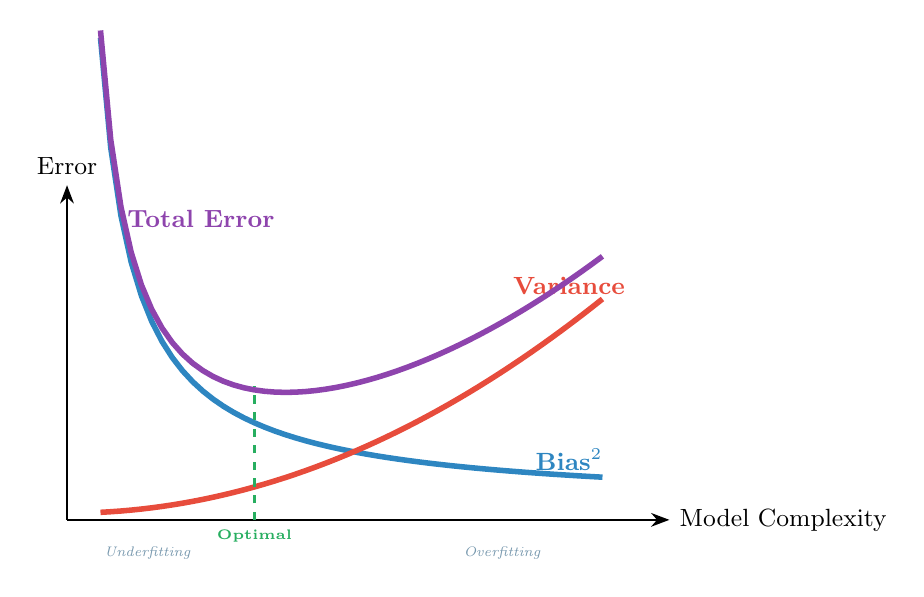
\begin{tikzpicture}[scale=0.85]
  \draw[-{Stealth}, thick] (0,0) -- (9,0) node[right, font=\small] {Model Complexity};
  \draw[-{Stealth}, thick] (0,0) -- (0,5) node[above, font=\small] {Error};

  % Bias curve (decreasing)
  \draw[very thick, secondary, line width=2pt, domain=0.5:8, samples=50] plot (\x, {3.5/\x + 0.2});
  \node[font=\small\bfseries, secondary] at (7.5, 0.9) {Bias$^2$};

  % Variance curve (increasing)
  \draw[very thick, accent, line width=2pt, domain=0.5:8, samples=50] plot (\x, {0.05*\x*\x + 0.1});
  \node[font=\small\bfseries, accent] at (7.5, 3.5) {Variance};

  % Total error
  \draw[very thick, purplehl, line width=2pt, domain=0.5:8, samples=50] plot (\x, {3.5/\x + 0.05*\x*\x + 0.3});
  \node[font=\small\bfseries, purplehl] at (2.0, 4.5) {Total Error};

  % Optimal point
  \draw[dashed, greenhl, thick] (2.8, 0) -- (2.8, 2.0);
  \node[font=\tiny\bfseries, greenhl, below] at (2.8, 0) {Optimal};

  % Underfitting / Overfitting labels
  \node[font=\tiny\itshape, primary!60] at (1.2, -0.5) {Underfitting};
  \node[font=\tiny\itshape, primary!60] at (6.5, -0.5) {Overfitting};
\end{tikzpicture}
\end{center}

\begin{itemize}[leftmargin=*]
  \item \textbf{Bias:} Error from oversimplified model (underfitting)---misses relevant relations.
  \item \textbf{Variance:} Error from model being too sensitive to training data (overfitting)---captures noise.
  \item \textbf{Goal:} Find the sweet spot that minimizes \emph{total error} (bias$^2$ + variance + irreducible error).
\end{itemize}

\subsection{Overfitting vs.\ Underfitting}

\begin{center}
\begin{tabular}{@{}p{6.5cm}p{6.5cm}@{}}
\toprule
\textbf{Underfitting (High Bias)} & \textbf{Overfitting (High Variance)} \\
\midrule
Model too simple & Model too complex \\
High training error, high test error & Low training error, high test error \\
Solution: more features, complex model, less regularization & Solution: more data, regularization, simpler model, dropout \\
\bottomrule
\end{tabular}
\end{center}

\subsection{Classification Metrics}

\begin{definitionbox}[Confusion Matrix]
A table summarizing classification results:
\begin{center}
\renewcommand{\arraystretch}{1.4}
\begin{tabular}{@{\hspace{6pt}}r@{\hspace{8pt}}l|c@{\hspace{12pt}}c@{\hspace{6pt}}}
  & & \multicolumn{2}{c}{\textbf{Predicted}} \\[2pt]
  & & \textbf{Positive} & \textbf{Negative} \\[1pt]
  \hline
  \multirow{2}{*}{\textbf{Actual}} & \textbf{Positive} & \textcolor{greenhl}{\textbf{TP}} & \textcolor{accent}{\textbf{FN}} \\[3pt]
  & \textbf{Negative} & \textcolor{accent}{\textbf{FP}} & \textcolor{greenhl}{\textbf{TN}} \\
\end{tabular}
\renewcommand{\arraystretch}{1.0}
\end{center}
\end{definitionbox}

\begin{itemize}[leftmargin=*]
  \item \textbf{Accuracy:} $\frac{TP + TN}{TP + TN + FP + FN}$ --- Overall correctness (misleading on imbalanced data).
  \item \textbf{Precision:} $\frac{TP}{TP + FP}$ --- Of predicted positives, how many are actually positive?
  \item \textbf{Recall (Sensitivity):} $\frac{TP}{TP + FN}$ --- Of actual positives, how many were correctly identified?
  \item \textbf{F1-Score:} $2 \cdot \frac{\text{Precision} \times \text{Recall}}{\text{Precision} + \text{Recall}}$ --- Harmonic mean of precision and recall.
  \item \textbf{ROC Curve:} Plot of TPR vs.\ FPR at various thresholds. \textbf{AUC} (Area Under Curve) summarizes performance.
\end{itemize}

\subsection{Regression Metrics}
\begin{itemize}[leftmargin=*]
  \item \textbf{MAE} (Mean Absolute Error): $\frac{1}{n}\sum|y_i - \hat{y}_i|$
  \item \textbf{MSE} (Mean Squared Error): $\frac{1}{n}\sum(y_i - \hat{y}_i)^2$
  \item \textbf{RMSE} (Root MSE): $\sqrt{\text{MSE}}$ --- same units as target.
  \item \textbf{$R^2$} (Coefficient of Determination): $1 - \frac{\sum(y_i - \hat{y}_i)^2}{\sum(y_i - \bar{y})^2}$ --- proportion of variance explained (1.0 = perfect).
\end{itemize}

\subsection{Cross-Validation}

\begin{definitionbox}[K-Fold Cross-Validation]
Split data into $k$ equally-sized folds. Train on $k-1$ folds, validate on the remaining fold. Repeat $k$ times, rotating the validation fold. Report the \textbf{average} performance across all $k$ folds.
\end{definitionbox}

\begin{center}
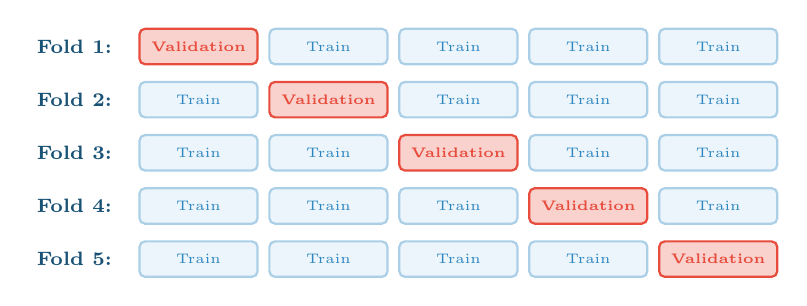
\begin{tikzpicture}[scale=0.75]
  \foreach \fold in {1,...,5} {
    \pgfmathsetmacro{\y}{-(\fold-1)*0.9}
    \node[font=\scriptsize\bfseries, primary, anchor=east] at (-0.3, \y) {Fold \fold:};
    \foreach \block in {1,...,5} {
      \pgfmathsetmacro{\x}{(\block-1)*2.2}
      \ifnum\block=\fold
        \fill[accent!25, rounded corners=2pt] (\x, \y-0.3) rectangle (\x+2, \y+0.3);
        \draw[thick, accent, rounded corners=2pt] (\x, \y-0.3) rectangle (\x+2, \y+0.3);
        \node[font=\tiny\bfseries, accent] at (\x+1, \y) {Validation};
      \else
        \fill[lightbg, rounded corners=2pt] (\x, \y-0.3) rectangle (\x+2, \y+0.3);
        \draw[thick, secondary!40, rounded corners=2pt] (\x, \y-0.3) rectangle (\x+2, \y+0.3);
        \node[font=\tiny, secondary] at (\x+1, \y) {Train};
      \fi
    }
  }
\end{tikzpicture}
\end{center}

%=============================================================
\section{Regularization Techniques}
%=============================================================

\begin{conceptbox}[Regularization]
Techniques to prevent overfitting by adding constraints or penalties to the model, discouraging complexity and improving generalization to unseen data.
\end{conceptbox}

\rowcolors{2}{white}{defbg}
\begin{longtable}{@{}p{3.5cm}p{10cm}@{}}
\toprule
\rowcolor{primary!15}
\textbf{Technique} & \textbf{Description} \\
\midrule
\endhead
L1 (Lasso) & Adds $\lambda\sum|w_i|$ to loss. Drives some weights to \textbf{exactly zero} (feature selection). \\
\addlinespace
L2 (Ridge) & Adds $\lambda\sum w_i^2$ to loss. Shrinks weights toward zero but doesn't eliminate them. \\
\addlinespace
Elastic Net & Combines L1 and L2: $\lambda_1\sum|w_i| + \lambda_2\sum w_i^2$. \\
\addlinespace
Dropout & Randomly deactivates neurons during training (neural networks). Prevents co-adaptation. \\
\addlinespace
Early Stopping & Stop training when validation error starts increasing. \\
\addlinespace
Data Augmentation & Artificially expand training data (rotations, flips, crops for images). \\
\addlinespace
Pruning & Remove branches from decision trees that provide little predictive power. \\
\addlinespace
Batch Normalization & Normalize layer inputs during training, stabilizes and speeds up learning. \\
\bottomrule
\end{longtable}

%=============================================================
\section{Practical Considerations}
%=============================================================

\subsection{Handling Imbalanced Data}
\begin{alertbox}[Class Imbalance]
When one class greatly outnumbers the other (e.g., 95\% negative, 5\% positive), models tend to predict the majority class and appear accurate while failing on the minority class.
\end{alertbox}

\textbf{Solutions:}
\begin{itemize}[leftmargin=*]
  \item \textbf{Resampling:} Oversampling minority (SMOTE), undersampling majority.
  \item \textbf{Class weights:} Assign higher cost to misclassifying minority class.
  \item \textbf{Evaluation:} Use Precision, Recall, F1, AUC instead of Accuracy.
  \item \textbf{Anomaly detection:} Treat minority class as anomalies.
\end{itemize}

\subsection{Hyperparameter Tuning}
\begin{itemize}[leftmargin=*]
  \item \textbf{Grid Search:} Exhaustively try all combinations of specified hyperparameter values.
  \item \textbf{Random Search:} Randomly sample combinations---often more efficient than grid search.
  \item \textbf{Bayesian Optimization:} Builds a probabilistic model to guide search toward promising regions.
  \item \textbf{Automated ML (AutoML):} Tools that automate model selection and tuning (e.g., Auto-sklearn, TPOT, H2O).
\end{itemize}

\subsection{Feature Importance and Interpretability}
\begin{itemize}[leftmargin=*]
  \item \textbf{Feature importance:} Random Forest and Gradient Boosting provide built-in scores.
  \item \textbf{SHAP (SHapley Additive exPlanations):} Model-agnostic explanations based on game theory.
  \item \textbf{LIME (Local Interpretable Model-agnostic Explanations):} Explains individual predictions.
  \item \textbf{Partial Dependence Plots:} Show the marginal effect of a feature on predictions.
\end{itemize}

%=============================================================
\section{Summary: Algorithm Selection Guide}
%=============================================================

\begin{center}
\small
\rowcolors{2}{white}{lightbg}
\begin{longtable}{@{}p{2.8cm}p{2.2cm}p{2.5cm}p{2cm}p{3.5cm}@{}}
\toprule
\rowcolor{primary!15}
\textbf{Algorithm} & \textbf{Type} & \textbf{Best For} & \textbf{Scalability} & \textbf{Key Strength} \\
\midrule
\endhead
Linear Regression & Regression & Linear relationships & High & Simple, interpretable \\
Logistic Regression & Classification & Binary classification & High & Probabilistic output \\
\addlinespace
Decision Tree & Both & Interpretable models & Medium & Easy to visualize \\
Random Forest & Both & General-purpose & High & Robust, feature importance \\
\addlinespace
XGBoost / LightGBM & Both & Tabular data & High & State-of-the-art accuracy \\
SVM & Both & Small-medium data & Low-Med & Effective in high dim \\
\addlinespace
KNN & Both & Small datasets & Low & No training phase \\
Na\"ive Bayes & Classification & Text classification & High & Very fast, simple \\
\addlinespace
K-Means & Clustering & Well-separated clusters & High & Simple, fast \\
PCA & Dim.\ Reduction & Preprocessing, viz & High & Captures max variance \\
\addlinespace
Neural Network & Both & Complex patterns & Varies & Universal approximator \\
CNN & Classification & Images, spatial data & GPU needed & Spatial feature learning \\
Transformer & Sequence & NLP, generative AI & GPU needed & Attention mechanism \\
\bottomrule
\end{longtable}
\end{center}

%=============================================================
\section{Best Practices Checklist}
%=============================================================

\begin{multicols}{2}
\begin{itemize}[leftmargin=1.5em, itemsep=2pt]
  \item[{\textcolor{greenhl}{\faIcon{check-circle}}}] Understand the problem type (classification, regression, clustering)
  \item[{\textcolor{greenhl}{\faIcon{check-circle}}}] Explore and visualize data before modeling (EDA)
  \item[{\textcolor{greenhl}{\faIcon{check-circle}}}] Handle missing values and outliers
  \item[{\textcolor{greenhl}{\faIcon{check-circle}}}] Encode categorical variables properly
  \item[{\textcolor{greenhl}{\faIcon{check-circle}}}] Scale/normalize features when required
  \item[{\textcolor{greenhl}{\faIcon{check-circle}}}] Split data into train/validation/test sets
  \item[{\textcolor{greenhl}{\faIcon{check-circle}}}] Start with simple baseline models first
  \item[{\textcolor{greenhl}{\faIcon{check-circle}}}] Use cross-validation for reliable estimates
  \item[{\textcolor{greenhl}{\faIcon{check-circle}}}] Tune hyperparameters systematically
  \item[{\textcolor{greenhl}{\faIcon{check-circle}}}] Monitor for overfitting (train vs.\ validation curves)
  \item[{\textcolor{greenhl}{\faIcon{check-circle}}}] Use appropriate metrics (not just accuracy)
  \item[{\textcolor{greenhl}{\faIcon{check-circle}}}] Address class imbalance if present
  \item[{\textcolor{greenhl}{\faIcon{check-circle}}}] Interpret and explain model decisions
  \item[{\textcolor{greenhl}{\faIcon{check-circle}}}] Document experiments and reproducibility
\end{itemize}
\end{multicols}

%=============================================================
\section{Common Pitfalls}
%=============================================================

\begin{alertbox}[Data Leakage]
Information from outside the training dataset unintentionally leaks into the model (e.g., using test data for feature scaling, target leakage). Leads to overly optimistic performance that fails in production.
\end{alertbox}

\begin{alertbox}[Not Enough Data]
Complex models (deep learning) require large amounts of data. Using them on small datasets leads to severe overfitting. Start simple.
\end{alertbox}

\begin{alertbox}[Ignoring Data Quality]
``Garbage in, garbage out.'' No algorithm can compensate for noisy, biased, or insufficient data. Invest in data cleaning and collection.
\end{alertbox}

\begin{alertbox}[Wrong Metric]
Using accuracy on imbalanced data, or MSE when outliers dominate. Always choose metrics aligned with the business objective.
\end{alertbox}

\begin{alertbox}[Correlation vs.\ Causation]
ML models find correlations, not causation. A model predicting outcomes does not mean the features \emph{cause} the outcome.
\end{alertbox}

%=============================================================
\section{ML Workflow --- End-to-End Example}
%=============================================================

\begin{conceptbox}[Predicting House Prices --- Workflow]
\begin{enumerate}[leftmargin=*, itemsep=2pt]
  \item \textbf{Define the problem:} Regression---predict continuous house price.
  \item \textbf{Collect data:} Dataset with features (area, bedrooms, location, age, etc.) and target (price).
  \item \textbf{EDA:} Visualize distributions, check correlations, identify missing values and outliers.
  \item \textbf{Preprocess:} Handle missing values (median imputation), encode categorical features (one-hot for location), scale numerical features (StandardScaler).
  \item \textbf{Split:} 80\% train, 20\% test; use 5-fold CV on training set.
  \item \textbf{Train baseline:} Linear Regression $\rightarrow$ evaluate RMSE, $R^2$.
  \item \textbf{Try advanced models:} Random Forest, XGBoost $\rightarrow$ compare metrics.
  \item \textbf{Tune:} RandomizedSearchCV on best model's hyperparameters.
  \item \textbf{Evaluate on test set:} Report final RMSE, MAE, $R^2$.
  \item \textbf{Interpret:} SHAP values to explain which features drive price predictions.
  \item \textbf{Deploy:} Save model (pickle/joblib), build API, monitor performance.
\end{enumerate}
\end{conceptbox}

%=============================================================
\section{Review Questions}
%=============================================================

\begin{enumerate}[leftmargin=*]
  \item Explain the difference between supervised, unsupervised, and reinforcement learning with examples.
  \item What is the bias--variance tradeoff? How does model complexity relate to underfitting and overfitting?
  \item Compare and contrast bagging and boosting. Name one algorithm for each.
  \item What is the purpose of cross-validation? Explain $k$-fold cross-validation.
  \item Define precision, recall, and F1-score. When would you prefer recall over precision?
  \item What is regularization? Compare L1 (Lasso) and L2 (Ridge) regularization.
  \item Explain how a decision tree makes predictions. What are Gini impurity and information gain?
  \item What is the kernel trick in SVM? Why is it useful?
  \item Describe the K-Means clustering algorithm and how to choose $k$.
  \item What is data leakage and how can it be prevented?
  \item Explain the architecture of a basic neural network (input, hidden, output layers, activation functions).
  \item How would you handle a dataset with 95\% negative and 5\% positive examples?
\end{enumerate}

\end{document}
